% \documentclass[UTF8]{article}
% 导言区
% % 导言区
% 中文支持
\usepackage[UTF8]{ctex}	
% pdf调用 封面
\usepackage{pdfpages}
% color宏包
\usepackage{color}  
% 导入图片
\usepackage{caption}
\usepackage{graphicx, subfig}
% 防止图片乱跑
\usepackage{float}
% 支持数学符号
\usepackage{amsmath}
% 支持代码块
\usepackage{listings}
% pdf加入大纲
\usepackage{hyperref}
% 大纲去红框
\hypersetup{hidelinks,
	colorlinks=true,
	allcolors=black,
	pdfstartview=Fit,
	breaklinks=true
}

% 绘制三线表
\usepackage{booktabs}    
% 消除警告
\usepackage{lmodern}

% 绘图
\usepackage{tikz}
\usetikzlibrary{positioning, shapes.geometric}
\tikzstyle{bag} = [align=center]

% 设置页面的环境,a4纸张大小,左右上下边距信息
\usepackage[a4paper, left=31.8mm, right=31.8mm, top=25.4mm, bottom=25.4mm]{geometry}

% 三线表内使用单元格
\usepackage{makecell}

% 设置页眉
\usepackage{fancyhdr} % Headers and footers
\usepackage{lastpage}
\pagestyle{fancy} % All pages have headers and footers
\fancyhead{} % Blank out the default header
\fancyhead[C]{网络过程控制系统课程报告:过程控制系统的智能化发展} % Custom header text

% 解决参考文献中作者名之间的连接词异常问题
\usepackage{gbt7714}
\bibliographystyle{gbt7714-numerical}


% 代码块的基本设置
\lstset{
 breaklines,%自动换行
 columns=fixed,       
 numbers=left,                                        % 在左侧显示行号
 numberstyle=\tiny\color{gray},                       % 设定行号格式
 frame=none,                                          % 不显示背景边框
 backgroundcolor=\color[RGB]{245,245,244},            % 设定背景颜色
 keywordstyle=\color[RGB]{40,40,255},                 % 设定关键字颜色
 numberstyle=\footnotesize\color{darkgray},           
 commentstyle=\it\color[RGB]{0,96,96},                % 设置代码注释的格式
 stringstyle=\rmfamily\slshape\color[RGB]{128,0,0},   % 设置字符串格式
 showstringspaces=false,                              % 不显示字符串中的空格
 language=python,                                        % 设置语言
}



% 两图片并排
% \begin{figure}[htbp]
% 	\centering
% 	\begin{minipage}{0.49\linewidth}
% 		\centering
% 		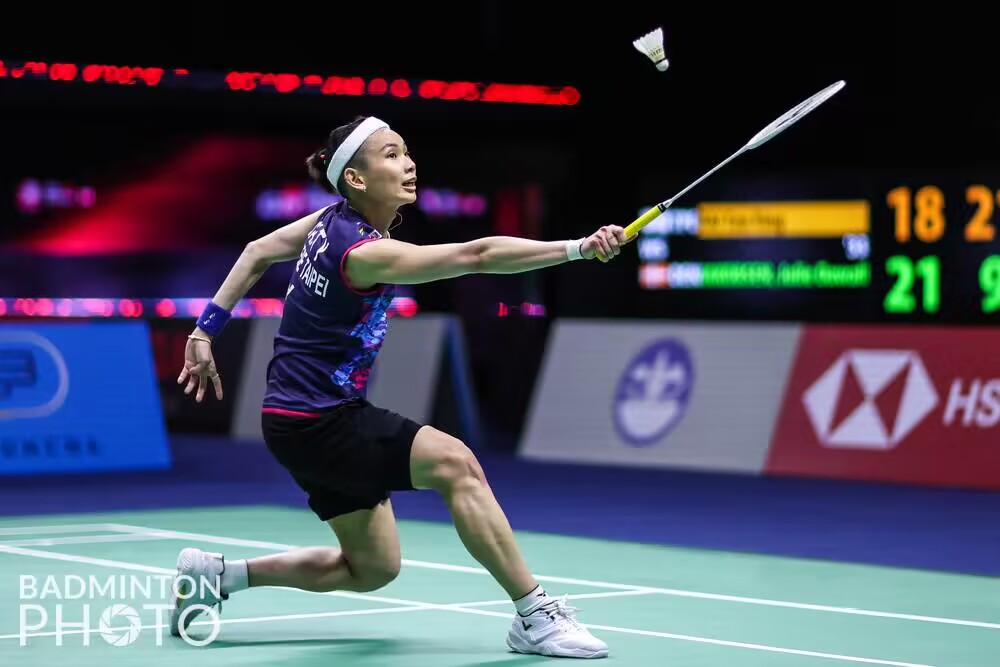
\includegraphics[width=0.9\linewidth]{figure/figure_1.jpg}
% 		\caption{title1}
% 		\label{label1} %文中引用该图片代号
% 	\end{minipage}
% 	%\qquad
% 	\begin{minipage}{0.49\linewidth}
% 		\centering
% 		
\includegraphics[width=0.9\linewidth]{figure/figure_3.jpg}
% 		\caption{title2}
% 		\label{label2} %文中引用该图片代号
% 	\end{minipage}
% \end{figure}


% 导入图片
% \begin{figure}[H]
%     \centering % 居中 
%     % 图片文件的相对路径
%     \includegraphics[width=.8\textwidth]{figure/exp1_1_model.png} 
%     \caption{Simulink模型} % caption是图片的标题
%     % \label{fig:img} % 此处的label相当于一个图片的专属标志,目的是方便上下文的引用
%     % 图片引用格式:\ref{fig:img} 可能需要二次编译
% \end{figure}

% 导入代码
% \begin{lstlisting}
% a
% \end{lstlisting}

% 重置章节编号
% \setcounter{section}{0}

% \begin{table}[H] % 防止表格乱跑
% \centering % 居中
% \begin{tabular}{cccccc} % 指明列数
% 	\toprule % 顶部粗线
% 	序号 & 姓名 & 性别 & 年龄 & 身高/cm & 体重/kg \\
% 	\midrule % 中间细线
% 	1 & 张三 & M & 16 & 163 & 50 \\ % 每行末尾都要加换行符
% 	2 & 王红 & F & 15 & 159 & 47 \\
% 	3 & 李二 & M & 17 & 165 & 52 \\
% 	\bottomrule % 底部粗线
% \end{tabular}
% \caption{title} % 标题
% \end{table}


% 上标形式的文献引用格式
% \textsuperscript{\cite{ref1}}
% \begin{thebibliography}{99}  
% 	\bibitem{ref1} 《现场总线技术及应用教程(第二版)》,王永华,机械工业出版社
%   \bibitem{ref13} \href{https://www.elecfans.com/kongzhijishu/1080520.html}{工业控制系统未来的发展趋势分析}:https://www.elecfans.com/kongzhijishu/1080520.html
% \end{thebibliography}

% \usepackage{my_package}

\documentclass{my_class}
% 在目录中section和页码之间添加引导点
\renewcommand{\cftsecleader}{\cftdotfill{\cftdotsep}}
% 目录居中
\renewcommand*\contentsname{\hfill 目录 \hfill}

% 报告正文字号为小四,中文宋体、英文Times New Roman;段落首行缩进2 字符,1.25倍行间距,无段前段后。图表中的字体与正文一致,字号比正文小半号(五号)。
\begin{document}
% \setmainfont{Times New Roman}
% \fontsize{12pt}{15pt}\selectfont

\begin{titlepage}
% 封面信息
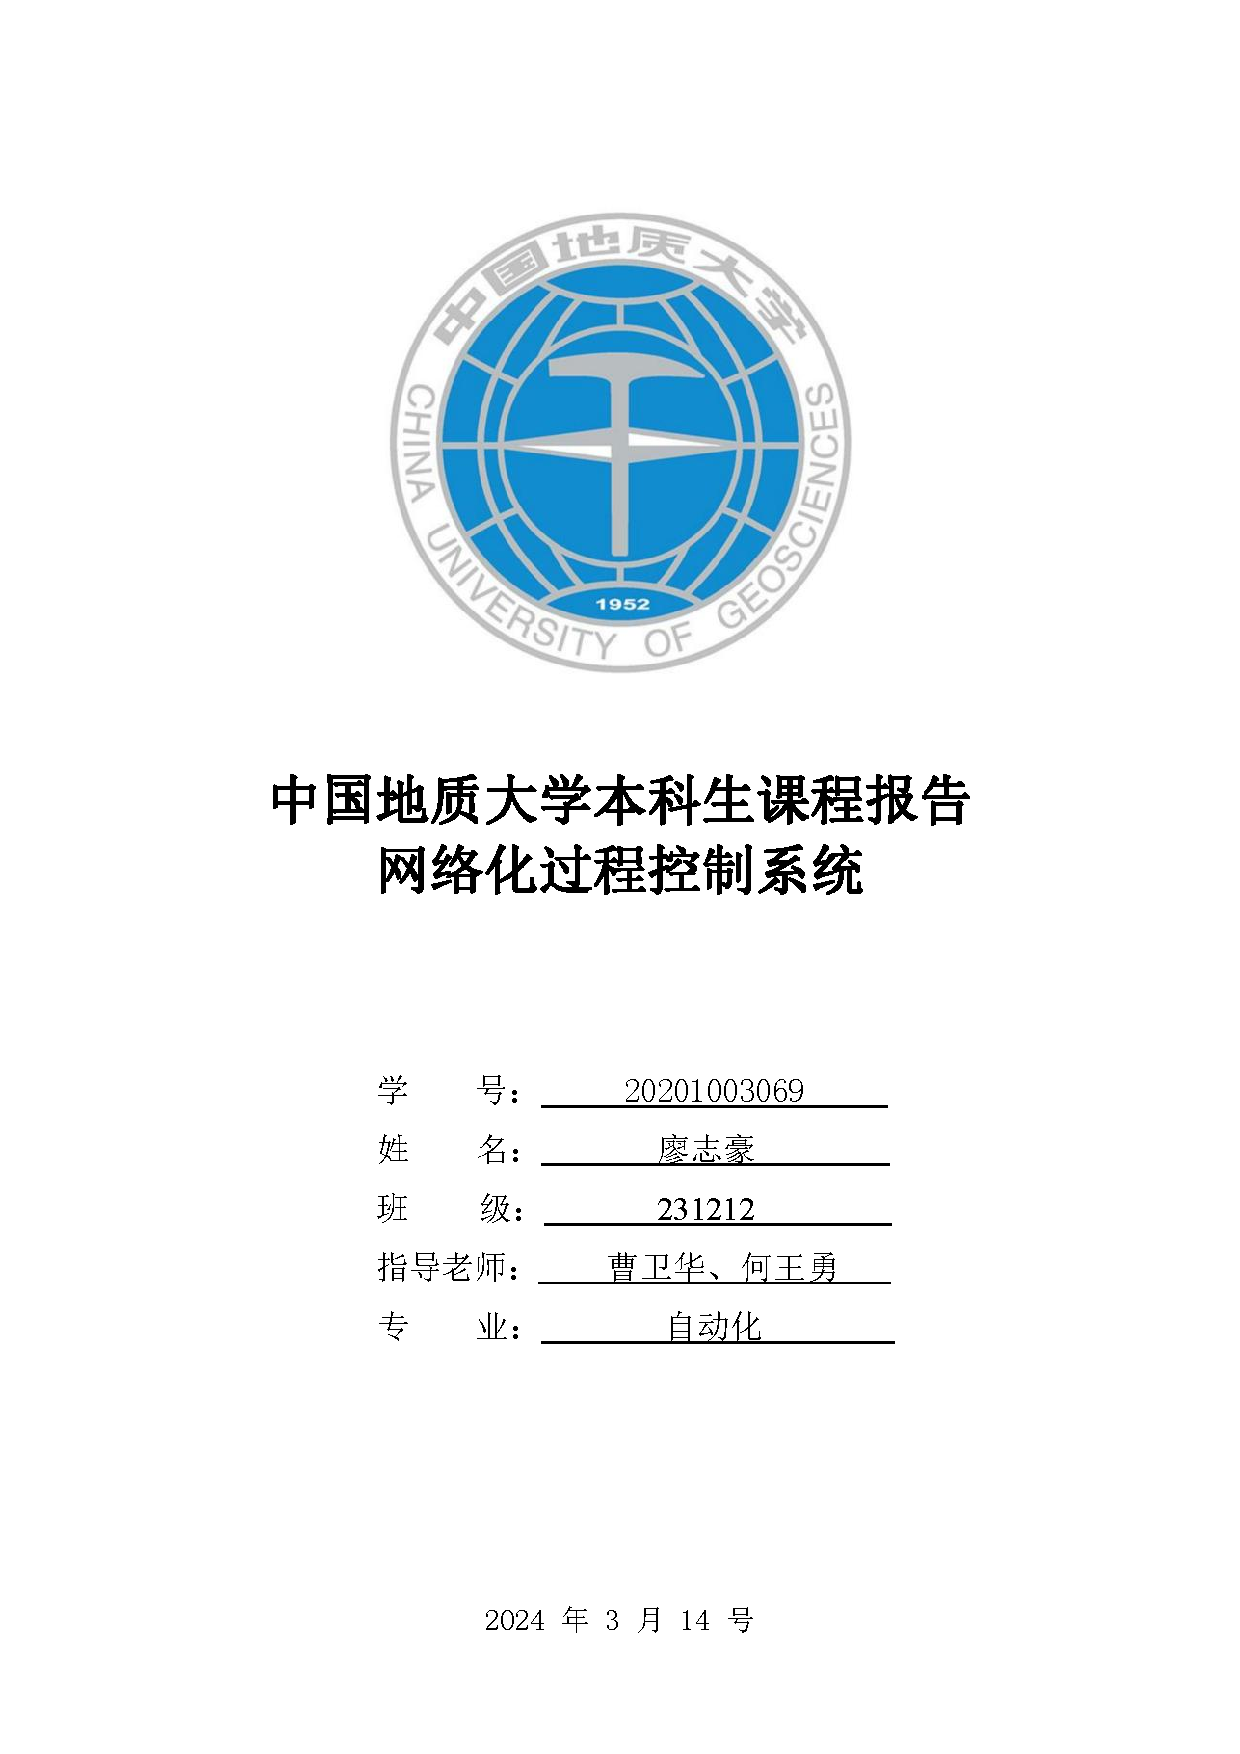
\includepdf[pages={1}]{./cover/cover.pdf}
\end{titlepage}

% 主题:过程控制系统的发展及展望
\begin{abstract}
	过程控制与过程控制系统在钢铁冶金、石油化工等工业生产领域中得到了广泛应用。随着以人工智能技术为代表的计算机技术的迅猛发展,工业过程控制领域的控制与决策方法也在逐渐出现智能化的技术创新,这进一步推动了过程控制系统的智能化。本文将对过程控制系统的发展历程做简要回顾,并针对过程控制系统智能化发展的现状和未来展望进行分析。

	\noindent \textbf{关键词}:过程控制系统;人工智能技术;智能化
\end{abstract}
\cleardoublepage

% 生成目录
\tableofcontents
\cleardoublepage

% 标题序号从0开始
\setcounter{section}{-1}
%
\section{引言}
以原材料生产为代表的过程工业是工业生产的主要类型之一\textsuperscript{\cite{PZKX201608005}}。作为过程工业的基础,过程控制与过程控制系统在钢铁冶金、石油化工等工业生产领域中得到了广泛应用。近年来,随着工业互联网、人工智能等技术的迅猛发展,工业过程控制领域也在发生一系列技术变革,这进一步推动了过程控制系统的智能化发展。本文将对过程控制系统的发展历程做简要回顾,并针对过程控制系统智能化发展的现状和未来展望进行分析。

%
\section{过程控制系统发展历程}

% 是什么?
过程控制是指工业生产过程中连续的或按一定周期程序运行的生产过程自动化\textsuperscript{\cite{2021过程控制系统}}。以过程控制为基础,过程控制系统结合了控制理论、计算机、网络通信等多种技术,能够满足实际的工业生产过程需求。

回顾历史,在工业生产需求的推动下,工业过程控制系统的发展与控制理论、计算机技术和网络通信技术等相关领域的发展密切相关。其中控制理论是理论设计基础,计算机技术是实现载体,网络通信技术则直接影响着过程控制系统的架构。过程控制系统的发展历程大致可以分为如下三个阶段\textsuperscript{\cite{过程控制的发展与展望}}:

\begin{table}[H] % 防止表格乱跑
\centering % 居中
\begin{tabular}{cccccc} % 指明列数
	\toprule % 顶部粗线
	阶段 & \makecell{第一阶段\\(70年代以前)} & \makecell{第二阶段\\(70 $\sim$ 80年代)} & \makecell{第三阶段\\(90年代以后)} \\
	\midrule % 中间细线
	控制理论 & 经典控制理论 & 现代控制理论 & \makecell{控制论、信息论、系统\\论、人工智能等学科交叉} \\
	控制工具 & \makecell{常规仪表\\(气动、液动、电动)} & 分布式控制计算机(DCS) & 计算机网络 \\
	控制要求 & 安全,平稳 & 优质、高产、低消耗 & \makecell{市场预测、快速响应、柔\\性生产、创新管理} \\
	控制水平 & 简单控制系统 & 先进控制系统 & 综合自动化(CIPS) \\
	\bottomrule % 底部粗线
\end{tabular}
\caption{过程控制发展的三个阶段} % 标题
\end{table}

%%
\subsection{第一阶段:集中式阶段}
70年代以前为过程控制系统发展的初级阶段,处于该阶段的过程控制系统以集中式过程控制系统为主,也可以看做是过程控制系统的最早形式。集中式过程控制系统前后经历了基地式仪表控制系统、单元组合式仪表控制系统、组装式仪表控制系统和集中式计算机控制系统等4个阶段。此外,过程控制所采用的控制理论在该时期也逐渐由经典控制理论向现代控制理论过渡。


%%
\subsection{第二阶段:网络化阶段}
70年代至80年代为发展阶段(网络化阶段),在该阶段由于计算机网络等通讯技术的迅速发展及其在工业过程控制中的应用,使得过程控制系统的发展逐步向网络化方向迈进,并最终产生了网络化过程控制系统。在这一演变过程中,先后出现了集散控制系统(DCS,又称分布式计算机控制系统)、现场总线控制系统、基于工业以太网的控制系统和流程工业综合自动化系统等4个发展阶段。此外,控制理论也逐渐转变为以现代控制理论为主导。

%%
\subsection{第三阶段:智能化阶段}
在90年代以后过程控制系统进入高级阶段(智能化阶段),在此阶段众多学科如控制论、信息论、系统论和人工智能等快速发展,为过程控制提供了进一步的理论基础。此外一些新兴技术如数据库、网络通讯技术等也为实现高水平的自动化控制提供了强有力的工具。该阶段的一个明显特征在于过程控制系统开始跳脱出传统过程控制的局限,发展出了一些更加有效的控制策略,即智能控制,由此过程控制系统开始向智能化方向发展。


%
\section{过程控制系统的现状分析}

%%
\subsection{人工智能与云计算技术}

近年来,随着通讯技术、人工智能以及云计算等技术的不断发展,过程控制系统的智能化也在不断推进。

一方面,智能传感器网络的出现使得可以更方便快捷地获取工业生产过程的各种运行数据,而物联网技术、工业互联网技术的出现和发展也使得生产企业能够对工业现场的生产设备信息、生产过程数据以及企业管理数据等海量数据进行实时的获取和存储。

在另一方面,基于云计算技术的工业云平台使得工业过程控制不再受限于计算机的算力,获得极为强大的计算能力和信息处理能力的支持\textsuperscript{\cite{ZGZZ2022S1004}}。在此基础上,将人工智能技术应用与工业过程控制成为了可能。在工业过程控制系统智能化的进程中,人工智能技术是不可或缺的一环。可以看到,人工智能技术的迅速发展为工业过程控制系统的智能控制以及智能决策等提供了大量工具\textsuperscript{\cite{MOTO202010002}},这对于构建决策和控制一体化的工业智能系统绝对是强有力的一股支持力量。近年来阿里云提出了“工业大脑”的概念,就是人工智能与云计算技术应用到工业生产中的极好例子。

\begin{figure}[H]
    \centering % 居中 
    % 图片文件的相对路径
    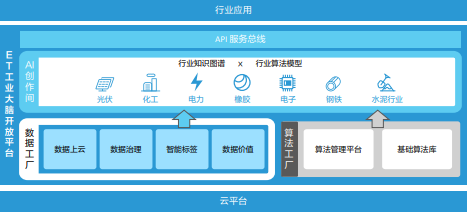
\includegraphics[width=.8\textwidth]{figure/工业大脑开放平台.png} 
    \caption{工业大脑开放平台} % caption是图片的标题
    % \label{fig:img} % 此处的label相当于一个图片的专属标志,目的是方便上下文的引用
    % 图片引用格式:\ref{fig:img} 可能需要二次编译
\end{figure}


%%
\subsection{数字孪生技术}

数字孪生(Digital Twin)技术最早由美国国防部提出,该技术通过建立真实飞机的数字模型,使用传感器实时获取实体飞机的物理数据,使得模型可以与真实飞机的状态完全同步。

利用数字孪生技术建立的数字模型可以反映物理实体的全生命周期过程,使得可以在虚拟世界中模拟物理实体的演化过程。将数字孪生模型与人工智能算法结合,还可以催生出更多更强大的工具。如美国通用电气公司为航空发动机构建的数字孪生模型,与人工智能算法结合后可以针对发动机故障进行预测,以减少检修维护成本。

\begin{figure}[H]
    \centering % 居中 
    % 图片文件的相对路径
    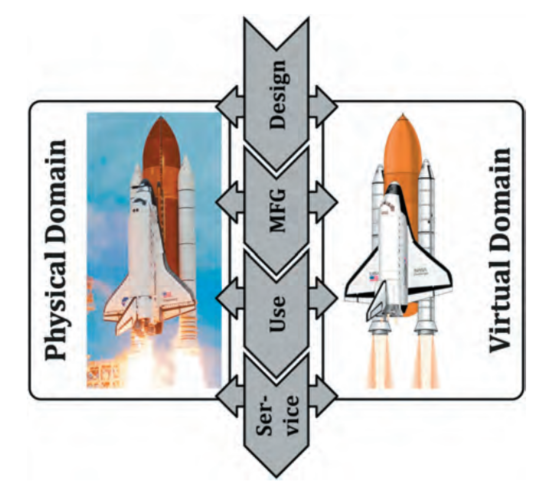
\includegraphics[width=.6\textwidth]{figure/数字孪生技术贯穿整个产品声明周期.png} 
    \caption{数字孪生技术贯穿整个产品声明周期\textsuperscript{\cite{GZDI202005001}}} % caption是图片的标题
    % \label{fig:img} % 此处的label相当于一个图片的专属标志,目的是方便上下文的引用
    % 图片引用格式:\ref{fig:img} 可能需要二次编译
\end{figure}

%%
\subsection{困难与挑战}
中国工业过程控制系统面临的困难和挑战包括:工业过程运行指标目标值范围的决策依赖于工艺工程师的经验,运行过程中的异常工况识别与处理需要依靠运行工程师的经验知识,这些问题的存在使得工业生产中各个工序控制系统的协同优化非常困难,从而难以实现生产指标的综合优化,导致工业过程中生产指标往往并非处于最优状态,甚至经常出现异常情况,造成了经济效益难以提高的局面。

上述问题的解决途径之一在于建立工业过程的智慧优化控制系统,主要包括智能优化决策系统\textsuperscript{\cite{MOTO201811002}}和智慧优化控制系统两个部分。智能优化决策系统针对的是工业过程决策,如生产制造全流程优化控制、过程工业资源计划调度等。该系统旨在使得工业生产能够自动获取市场需求变化和资源供给等方面的数据,并对这些信息能够自主学习和决策,以优化资源的配置,同时对工业生产过程进行综合分析,给出经过优化后的运行指标目标值。智慧优化控制系统针对工业过程控制,旨在使系统能够自动感知生产条件变化,通过自适应控制等方式实现运行指标的优化控制;同时可以对工况进行实时监视,能够及时诊断异常工况并采取排除措施。

%
\section{未来发展方向展望}
随着现代信息技术和工业自动化技术的不断融合,中国工业过程控制系统的未来呈现出广阔的发展前景。个人认为在未来中国工业过程控制系统有以下几个关键的发展方向:

智能化:智能化将成为驱动工业过程控制系统发展的核心力量。借助于人工智能、大数据分析、云计算等先进技术,未来的工业过程控制系统将具备更强的数据处理能力和智能决策能力,实现生产过程的优化调整和资源配置的最大化效率。

信息化:信息化与工业化的深度融合将是未来发展的重点之一。通过构建集成化的信息物理系统(CPS),实现机器间的互联互通,以及生产数据和管理数据的无缝对接,从而提升整个生产系统的透明度和灵活性。

数字化:以数字孪生技术为代表的计算机仿真技术将大大简化工业过程控制系统的设计流程及运营工作,包括但不局限于工业生产过程控制、生产指标综合决策优化等等。

绿色制造与可持续发展:环境友好和可持续发展理念也将渗透到工业过程控制系统的设计和运营之中。节能减排、绿色制造和循环经济的理念将引导企业采用更为环保的控制技术和材料,同时优化生产过程以减少对环境的负面影响。

展望未来,中国工业过程控制系统的发展将是一个多元化、综合化、智能化的过程。为了更好地面对全球化挑战,提高自身的国际竞争力,中国工业过程控制系统需要不断提升产品和服务质量,加强国际合作和交流,积极参与国际标准的制定。同时,通过技术创新和产业升级,中国有望在全球工业自动化领域占据更为重要的地位,并为推进世界工业生产的智能化和数字化作出重要贡献。


% unsrt:保持引用次序
% \bibliographystyle{unsrt}
\bibliographystyle{gbt7714-numerical}
% % 插入ref.bib文件
\bibliography{ref}


% \begin{thebibliography}{99}  
% 	\bibitem{ref1} 柴天佑.工业过程控制系统研究现状与发展方向[J].中国科学:信息科学,2016,46(08):1003-1015.

% 	\bibitem{ref2} 曹卫华,何王勇,甘超.过程控制系统[M].中国地质大学出版社:武汉.

% 	\bibitem{ref3} 柴天佑.自动化科学与技术发展方向[J].自动化学报,2018,44(11):1923-1930.DOI:10.16383/j.aas.2018.c180252.

% 	\bibitem{ref4} 黄海松,陈启鹏,李宜汀等.数字孪生技术在智能制造中的发展与应用研究综述[J].贵州大学学报(自然科学版),2020,37(05):1-8.DOI:10.15958/j.cnki.gdxbzrb.2020.05.01.

% 	\bibitem{ref5} 金以慧,王诗宓,王桂增.过程控制的发展与展望[J].控制理论与应用,1997(2):145-151.

% 	\bibitem{ref6} 柴天佑. 工业人工智能发展方向. 自动化学报, 2020, 46(10): 2005−2012 doi:  10.16383/j.aas.c200796

% 	\bibitem{ref7} 张梦,郭大亮,童欣等.现代造纸企业数字化过程控制系统的研究进展[J].中国造纸,2022,41(S1):16-22.
% \end{thebibliography}

\end{document}